\documentclass[a4paper,11pt]{article}

\usepackage[spanish]{babel}
\usepackage[T1]{fontenc}
\usepackage[utf8]{inputenc}
\usepackage{textcomp}
\usepackage{amsmath}
\usepackage{amsfonts}
\usepackage{amssymb}
\usepackage{fancyhdr}
\usepackage{anysize}
\usepackage{graphicx}

\begin{document}

\marginsize{2cm}{2cm}{2cm}{2cm}
\renewcommand\contentsname{Indice}
\renewcommand{\footrulewidth}{0.4pt}
\renewcommand{\headrulewidth}{0.4pt}

\pagestyle{empty}

\includegraphics[scale=0.3]{logo.png}

\begin{center}
	\Huge{Algoritmos y Programación II}\\
	\Huge{TP 3}\\
\end{center}
\vspace{4cm}

\begin{center}
	\begin{tabular}{|c|c|c|}
		\hline
		\textbf{Nombre}  & \textbf{Padrón}\\
		\hline
		 \hspace{6cm}  & \hspace{3cm}\\
		 \hline
		 Jose Paz & 91841   \\
		 \hline		 
	\end{tabular}
\end{center}

\vfill 

\begin{flushleft}
	\Large{Docente: Andres }\\
	\Large{Cuatrimestre: Primero}\\
	\Large{Año: 2020}\\
\end{flushleft}


\newpage
\setcounter{page}{1}

\section{Diagramas UML}
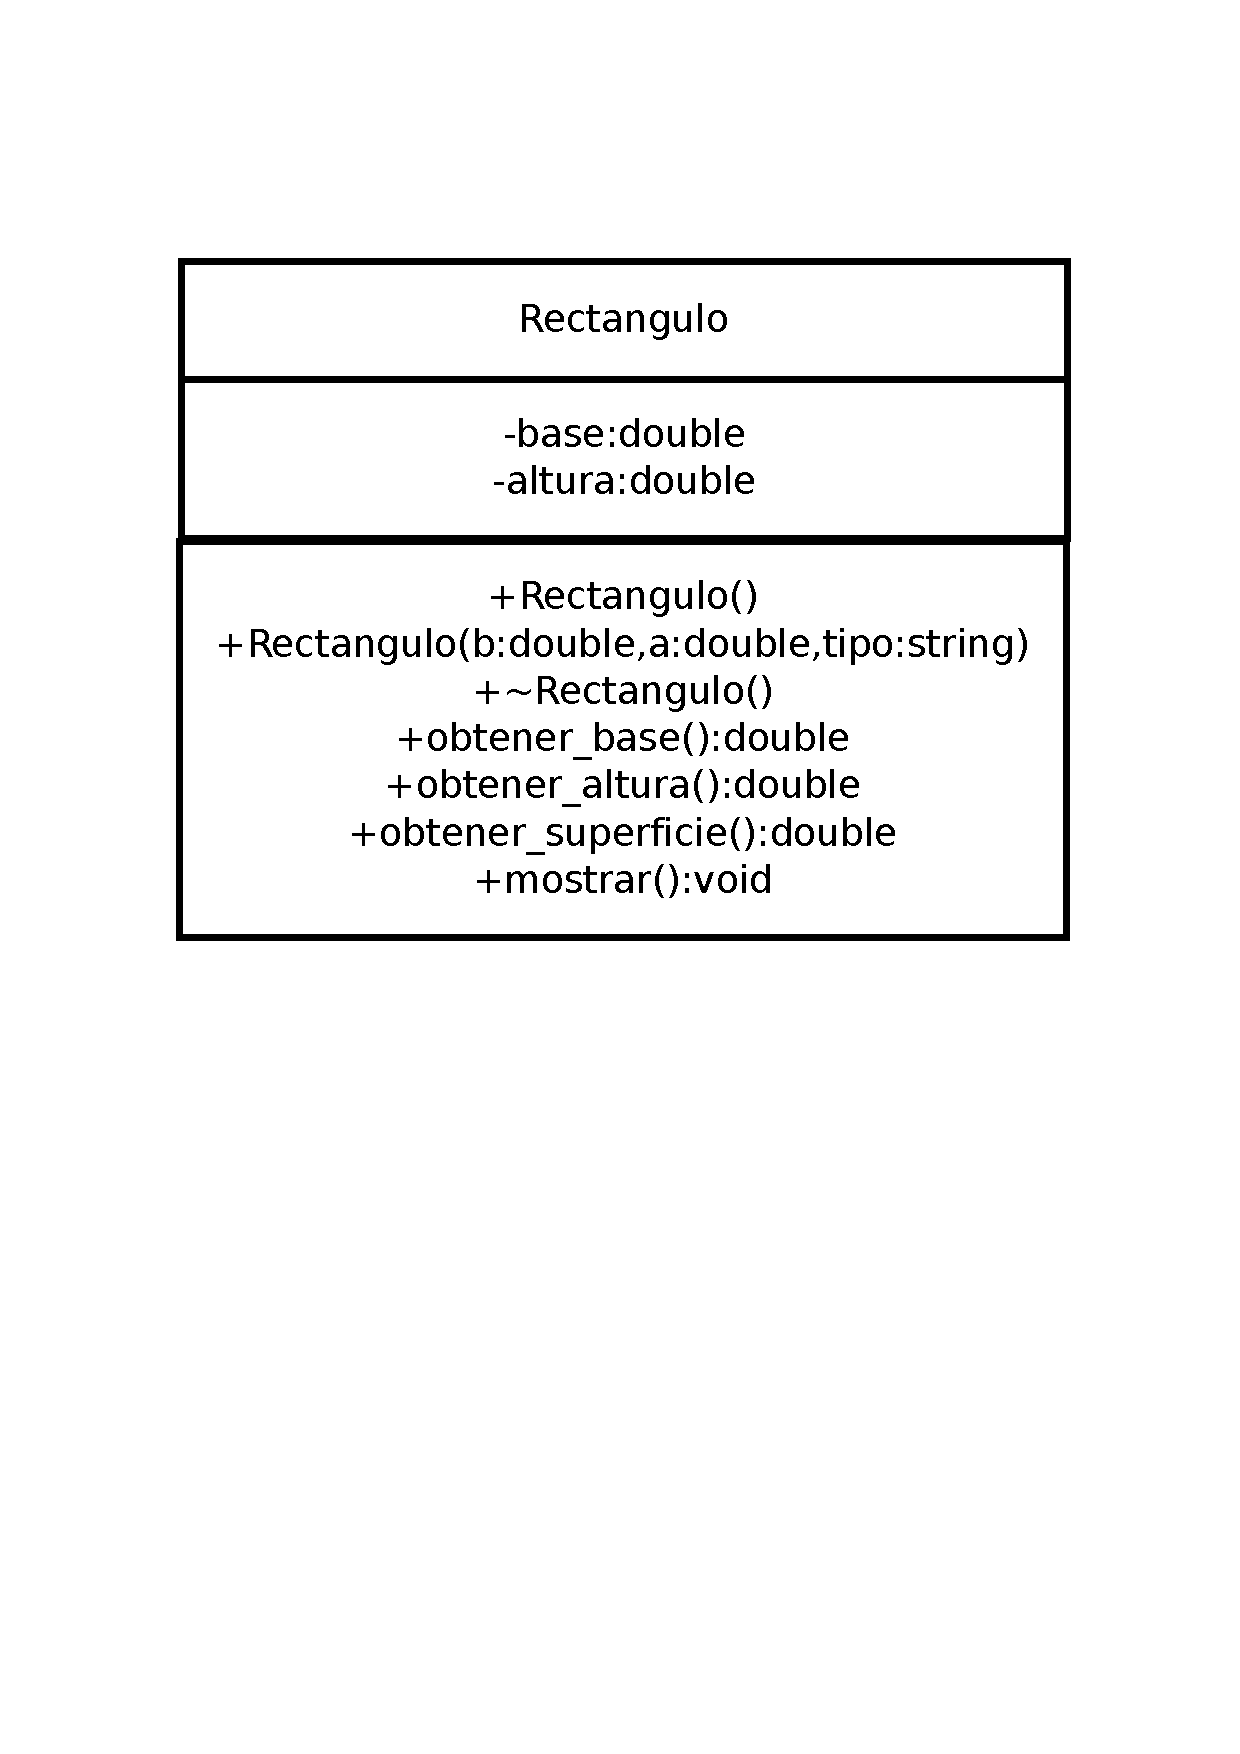
\includegraphics[scale=0.3]{rectangulo.pdf}



\end{document}


